\section{Simulator}

In this section, we will introduce our simulator.
It is included achieve the cashier-free supermarket in Unity3D, and the item recognition method what we use, then we combine them into a whole and application of simulation in real scene.

\subsection{Scene simulation}

We use Unity3D to simulate scene like a truth supermarket, the model is basic on the layout of Supermarket after our investigation.
It is length and width and height of the scene are 40m, 25m, 6m, and aisle width is 2.7m.
In the scene we set 5 bins,and each of bin width is 2.35m and height is 1.7m.
Then we put the cameras on the bins. 
We put the each camera on the bins which height is 2.22m, and set cameras 6.8m apart from the previous calculations.
Then we put four-direction cameras on the aisle, which is placed every three meters above the corridor. 
A four-direction camera has 4 cameras for 4 directions, and we put them on the 3.5m. height of aisle. 
In the scene we built, we totaly use 152 cameras in this scene.
There is shown in the figure.6.
\begin{figure}[htbp]
\centerline{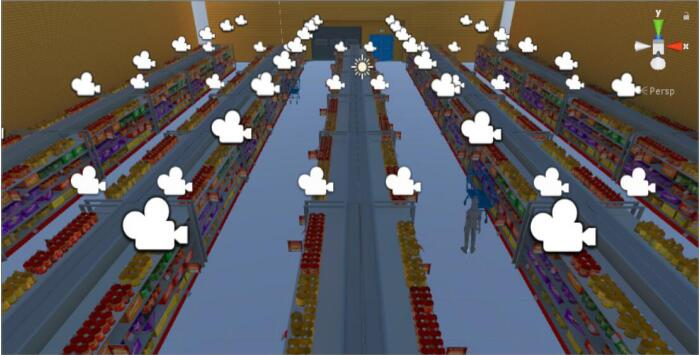
\includegraphics[width=7cm,scale=0.8]{supermarket.jpg}}
\caption{Page Size and Optical Resolution}
\label{fig}
\end{figure}

After calculation and field investigation, we draw the h-fov is 1.2 bin is best for catching the maximum range and clearer picture, and the each camera can cover 2 bin.
In figure.7, we can see the cameras which on shelves can clearly obtain the type and quantity of goods, this provides a great help for our later identification.
\begin{figure}[htbp]
\centerline{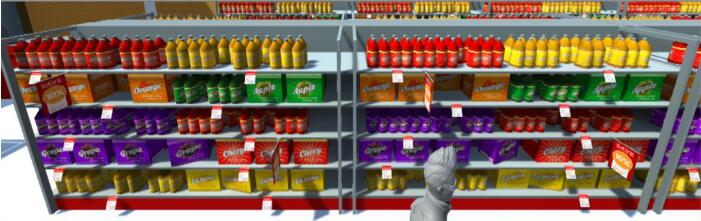
\includegraphics[width=7cm,scale=0.8]{shelves.jpg}}
\caption{Page Size and Optical Resolution}
\label{fig}
\end{figure}

In this scene, we can calculate the location of the camera in the real scene and the number of cameras needed.
In Unity3D we can use the clear screenshot F9 to get the picture which is describe the items type and quantity on shelves, and it is resolution is 1600*1200.
We will use pictures what we get to do item recognition and identify their type and number.
Then we will apply the simulated scene to the real scene. 

\subsection{Item Recognition}
In this section, we will introduce how we do item recognition and recognized results 
The item recognition system is dependent on YOLOv3 method.
And in our Simulator, we use OpenCV3.40 and CUDA8.0. to achieve it, they are better suited for image processing systems. 
Then we search some sample pictures from Internet as our experimental pictures to verify the feasibility of the system.
There is a picture about Yakult which we get in web, and then we put it in the identity system what we build based on YOLOv3\cite{yolov3}. As for figure.8, we can accurately identity the types of articles and number of articles, it uses boxes to present items tested.
\begin{figure}[htbp]
\centerline{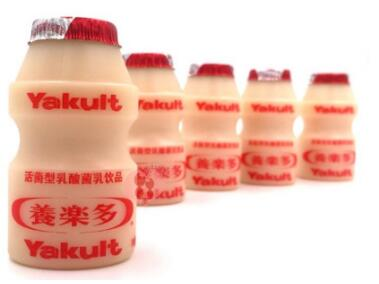
\includegraphics[width=3.5cm,scale=0.6]{Yakult.jpg} 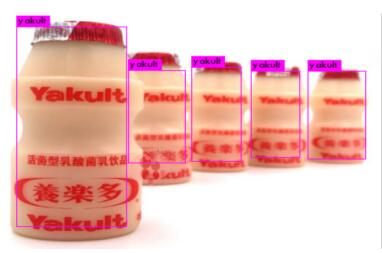
\includegraphics[width=3.5cm,scale=0.6]{Yakult_new.jpg}}
\caption{.}
\label{fig}
\end{figure}

Their recognition rates ranged from left to right is 100, 86, 100, 100, 100.
This proves the feasibility of our system.

Then we trained more items in our system.
These pictures were taken from real supermarkets.
In order to verify the accuracy of this system, we have selected a number of categories to train, and randomize them to verify accuracy.
In figures.9, there are different types and quantities, we can accurately identify their types and quantities by our system.
%\begin{figure}[htbp]
%\centerline{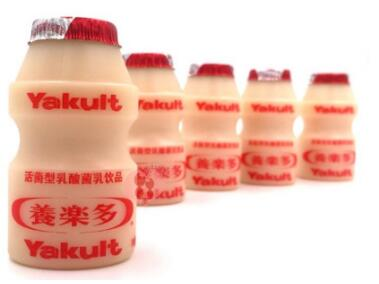
\includegraphics[width=3.5cm,scale=0.6]{Yakult.jpg} 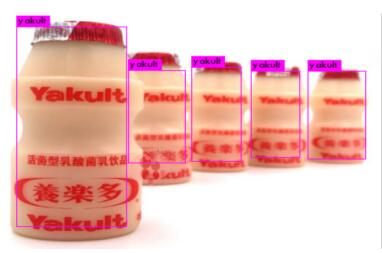
\includegraphics[width=3.5cm,scale=0.6]{Yakult_new.jpg}}
%\caption{.}
%\label{fig}
%\end{figure}

This proves our item recognition can be used in real scenes with high accuracy.
Ultimately we'll have it with multi cameras to achieve cashier-free supermarket.
